\documentclass[12pt]{scrartcl}

\usepackage[english]{babel}
\usepackage[T1]{fontenc}
%\usepackage[noadjust]{cite}
\usepackage{url,color} % Citation numbers being automatically sorted and properly "compressed/ranged".
\usepackage{graphics,amsfonts}
\usepackage{epstopdf}
\usepackage[pdftex]{graphicx}
\usepackage[cmex10]{amsmath}
\usepackage{physics}
% Also, note that the amsmath package sets \interdisplaylinepenalty to 10000
% thus preventing page breaks from occurring within multiline equations. Use:
\interdisplaylinepenalty=2500
% after loading amsmath to restore such page breaks as IEEEtran.cls normally does.
\usepackage[utf8]{inputenc}
% Useful for displaying quotations
%\usepackage{csquotes}
% Compact lists
%\let\labelindent\relax
\usepackage{enumitem}
\usepackage{hhline}
\usepackage{wrapfig}
\usepackage{makecell}

\usepackage[bookmarksopen=false]{hyperref}
\usepackage{bookmark}
\usepackage[style=alphabetic,backend=biber]{biblatex}

%tikz figures
\usepackage{tikz}
\usetikzlibrary{automata,positioning,chains,shapes,arrows}
\usepackage{pgfplots}
\usetikzlibrary{plotmarks}
\newlength\fheight
\newlength\fwidth
\pgfplotsset{compat=newest}
\pgfplotsset{plot coordinates/math parser=false}

\usepackage{array}
% http://www.ctan.org/tex-archive/macros/latex/required/tools/
%\usepackage{mdwmath}
%\usepackage{mdwtab}
%mdwtab.sty	-- A complete ground-up rewrite of LaTeX's `tabular' and  `array' environments.  Has lots of advantages over
%		   the standard version, and over the version in `array.sty'.
% *** SUBFIGURE PACKAGES ***
%\usepackage[tight,footnotesize]{subfigure}
\usepackage{subfig}

\usepackage[top=1.5cm, bottom=2cm, right=1.6cm,left=1.6cm]{geometry}
\usepackage{indentfirst}

\usepackage{times}
% make sections titles smaller to save space
%\usepackage{sectsty}
%\sectionfont{\large}
% enable the use of 'compactitem', a smaller 'itemize'
%\usepackage{paralist}

% to split equations using dmath env
\usepackage{breqn}
% nice rules in tables
%\usepackage{booktabs}
\usepackage{tabu}
\usepackage{array}

% tabular positioning
\usepackage{dblfloatfix}
\usepackage{lipsum}

% for simil-Times New Roman
\usepackage{mathptmx}% http://ctan.org/pkg/mathptmx
% for inteline spacing
\linespread{1.5}



% bibliography
\addbibresource{tex/bibliography.bib}

\begin{document}
%\maketitle


\begin{titlepage}
	
\centering
{\includegraphics[width=4cm]{img/logo_unipd}
\hspace{7cm}
\includegraphics[width=4cm]{img/logo_dei}
}

\vspace{2cm}
{\bfseries\Large\textit
	Wireless Communications\\
} 
{\bfseries\Huge
	Simulation of Multipath Fading Channels\\
}
\vspace{1cm}
{\large
	\textbf{Author:}
	
	\vspace{5mm}
	
	\normalsize
	\begin{tabular}{ll}
		Mattia Lecci 	& {\footnotesize\textit{(1153428)}} \\ 
	\end{tabular} 
} 
\vfill

% total: min 5, max 15 pages
\begin{abstract}	% max 10 lines
{\Large\textbf{Abstract}}
\vspace{0.5cm}

Throughout the years, many wireless channel simulators have been proposed with different performance objectives. In this project I will implement 8 of them, explaining how they work, the differences from one another and, finally, testing statistical and computational performance, comparing all of them in order to find their strengths and weaknesses.

As expected, there is no single winner, but two of them will show appreciable characteristics in separate performance indexes. You will see how the fastest performer will present below average statistical properties and how, maybe surprisingly, the original Clarke's model will actually yield the best overall statistical performance with a speed comparable to more modern solutions

\end{abstract}

\end{titlepage}
\newpage
\section{Introduction} % max 1 page
\label{sec:introduction}

Since the Seventies, simulating a good wireless channel was recognized to be fundamental for wireless systems design. It was acknowledged right from the start for being simpler, cheaper and more repeatable than a channel sounding: no external expensive gear was required and a new simulation could be done in a matter of seconds or less.

Early on, a simple yet fairly realistic channel model was presented by Clarke \cite{clarke}, on which all the subsequent simulators were based on and many different statistics were extrapolated. A few years later, Jakes created the de facto standard simulator \cite{jakes} for many years to follow. His proposal was to artificially impose certain simmetries to how the channel behaves, thus being able to simulate an approximation of Clarke's model but only with a fouth of the oscillators. Jakes' approach, though, had some problems and throughout the years many proposals (\cite{A1},\cite{A2},\cite{A3},\cite{C1},\cite{C2}) have been done in order to fix most, if not all of them.

Finally, while proposing a new simulator, \textit{Xiao, Zheng} and \textit{Beaulieu} \cite{B1} recognized how well \textit{Clarke}'s model actually beahves even with a low number of sinusoidal components. In fact, they proved how fast it converges to the ideal formulas, thus not needing as much oscillators as \textit{Jakes} (and all those that followed) actually thought.

The report is structured as follow: in Section \ref{sec:technical_approach} I will present the technical aspects of the project, starting from Subsection \ref{subsec:objectives} which delineates the main objectives, then in Subsection \ref{subsec:math_models} the mathematical models of all the implemented simulators will be carefully described and in Subsection \ref{subsec:scenario} an outline of the code structure will be presented. Finally, in Subsection \ref{subsec:complications} I will briefly talk about a few complications encountered while completing this project. In Section \ref{sec:results}, then, the results will be presented and lastly in Section \ref{sec:conclusions} the conclusions will be drawn.
\newpage
\section{Technical Approach}	% no limits given
\label{sec:technical_approach}

In this Section all the technical aspects of the project will be presented. A quick explanation of the various simulators implemented will follow in Subsection~\ref{subsec:math_models}, following the history of the subject. That is the reason why the order of the citations will be different from the one proposed. Note that all of the equations have been slightly modified in order to obtain unit power fading channels.


\subsection{Objectives} % max 5 lines
% what you want to show
\label{subsec:objectives}

The main objective of this project is to evaluate the performance of different types of wireless channel simulators. In particular, I'm interested, here, in simulating a Rayleigh fading channel, namely a channel where no \textit{Line-Of-Sight} (\textit{LOS}) component is present. I will show both statistical and performance results for all of the 8 simulators implemented, comparing them to one another.
\subsection{Mathematical models used} % no limits given
\label{sec:math_models}


\subsection{Scenario and Implementation} % max 20 lines
\label{subsec:scenario}

The project has been implemented using MATLAB\textsuperscript{\textregistered} R2017a.

A separate function for each simulator has been created as well as the interface \texttt{createChannel} to create a realization of a channel with all different kinds of parameters, such as $f_d,\ T$, duration (either in number of samples, seconds or multiples of $T_{coh}$), type of simulator, number of oscillators (i.e. the parameter $M \approx N/4$ for most simulators), number of independent channels and the interpolation method for the Komninakis simulator (either by \texttt{filter}, \texttt{spline}, \texttt{pchip} or \texttt{linear} interpolation). For what concerns the Komninakis simulator, shaping filter's coefficients were taken from \cite[p.~317]{digital} which assumes $f_dT_p=0.1$.

Separate functions for the computation of all the statistics required have been done and again all of them have multiple optional parameters to be set. Note that when talking about correlation I mean the statistical, not the temporal one. Hence, I also created a function that computes an estimate of the statistical correlations (all of those described in Eqs.~\ref{eqs:correlations}) given a number of independent channels (which can be easily created exploiting the Name-Value parameter \texttt{NChannels} from the function \texttt{createChannel}). The only exception to this rule is \textit{Jakes}' simulator since it's fully deterministic. The standard temporal correlation has been used in this specific case.

More functions were created in order to properly and simply plot all of the numerous statistics and to ensure a homogeneous look. Finally, different \texttt{mains} were created to obtain different types of results in an orderly manner and the possibility to store and load statistics has been added in order to promptly plot previously computed statistics.
\subsection{Complications found} % max 5 lines
\label{sec:complications}


\section{Results} % min 7 pages
\label{sec:results}

%%%%%%%%%%%%%%%%%%%%%%%%%%%%%%%%%%%%%%%%%%%%%%%%%%%%%%%%%%%%%%%%%%%%%%%%%%%%%%%%%%%%%%%%%%%%%%%
%%%%%%%%% PDFs
%%%%%%%%%%%%%%%%%%%%%%%%%%%%%%%%%%%%%%%%%%%%%%%%%%%%%%%%%%%%%%%%%%%%%%%%%%%%%%%%%%%%%%%%%%%%%%%
\begin{figure}
\hfill
\begin{minipage}{.45\linewidth}
	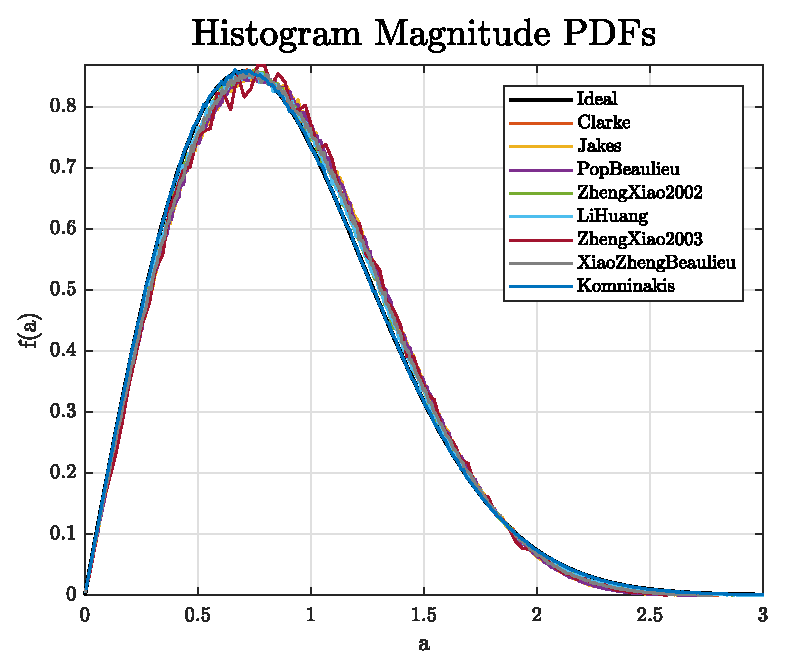
\includegraphics[width=\linewidth]{img/histMag.eps}
\end{minipage}
\hfill
\begin{minipage}{.45\linewidth}
	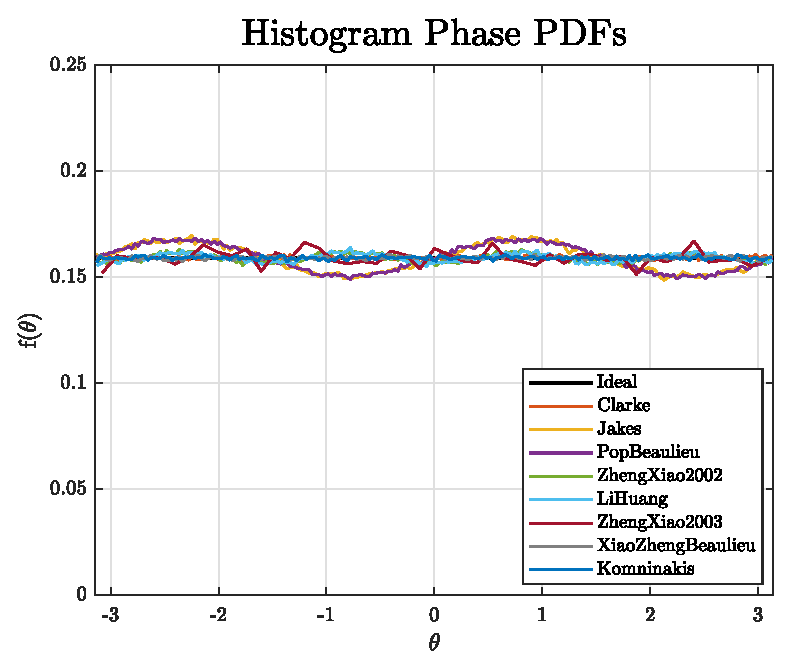
\includegraphics[width=\linewidth]{img/histPhase.eps}
\end{minipage}
\hfill

\caption{Histograms of Magnitudes and Phases of all the implemented simulators. Note the aforementioned problem with ZhengXiao2003}
\label{fig:histograms}
\end{figure}

Note that ZhengXiao2003 has a particularly zigzagy line since the first few samples did not respect the distributions. Computing more samples, then, didn't allow me to create as many channels as for the others due to memory limitations.

%%%%%%%%%%%%%%%%%%%%%%%%%%%%%%%%%%%%%%%%%%%%%%%%%%%%%%%%%%%%%%%%%%%%%%%%%%%%%%%%%%%%%%%%%%%%%%%
%%%%%%%%%%%% Correlations
%%%%%%%%%%%%%%%%%%%%%%%%%%%%%%%%%%%%%%%%%%%%%%%%%%%%%%%%%%%%%%%%%%%%%%%%%%%%%%%%%%%%%%%%%%%%%%%

\begin{figure}
	\hfill
	\begin{minipage}{.45\linewidth}
		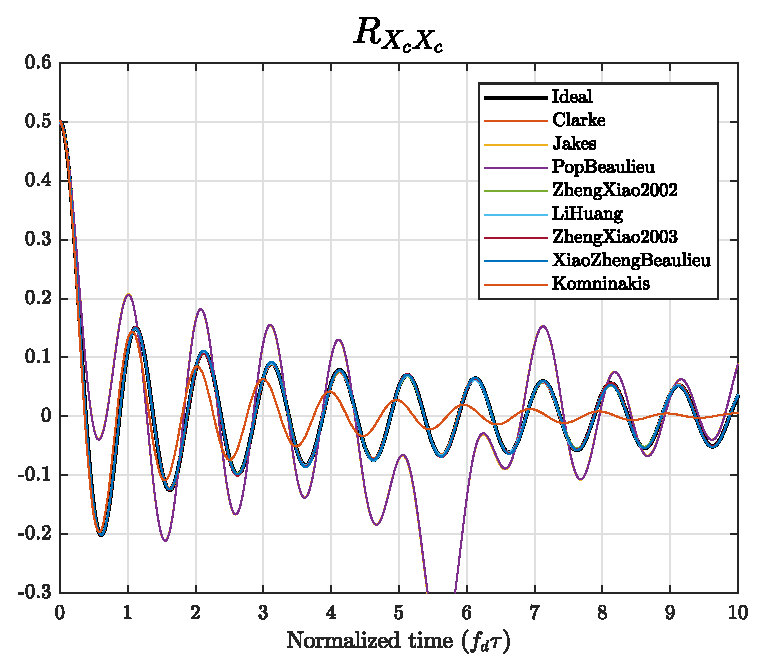
\includegraphics[width=\linewidth]{img/XcXc.eps}
	\end{minipage}
	\hfill
	\begin{minipage}{.45\linewidth}
		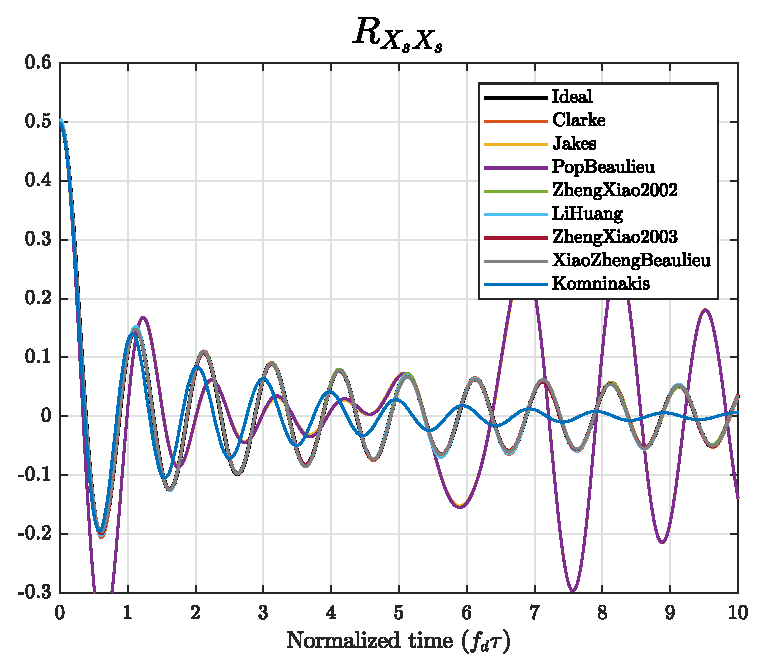
\includegraphics[width=\linewidth]{img/XsXs.eps}
	\end{minipage}
	\hfill
	
	\vspace{2mm}
	
	\hfill
	\begin{minipage}{.45\linewidth}
		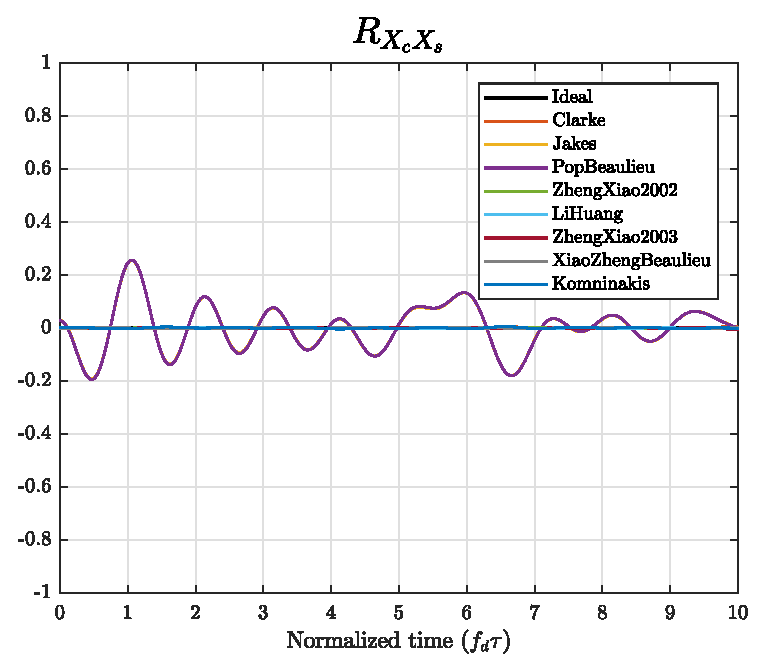
\includegraphics[width=\linewidth]{img/XcXs.eps}
	\end{minipage}
	\hfill
	\begin{minipage}{.45\linewidth}
		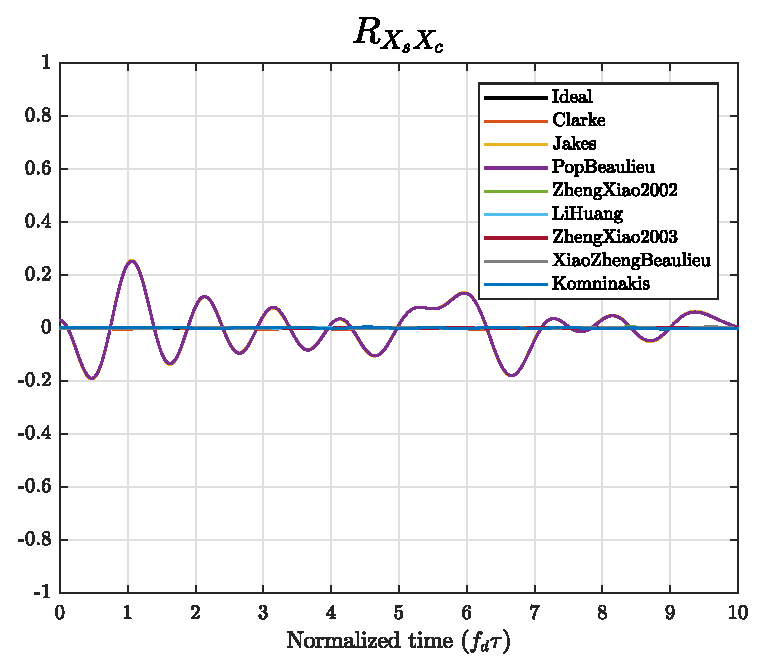
\includegraphics[width=\linewidth]{img/XsXc.eps}
	\end{minipage}
	\hfill
	
	\caption{Cross correlations between real and imaginary components}
	\label{fig:4xcorr}
\end{figure}

\begin{figure}
	\hfill
	\begin{minipage}{.32\linewidth}
		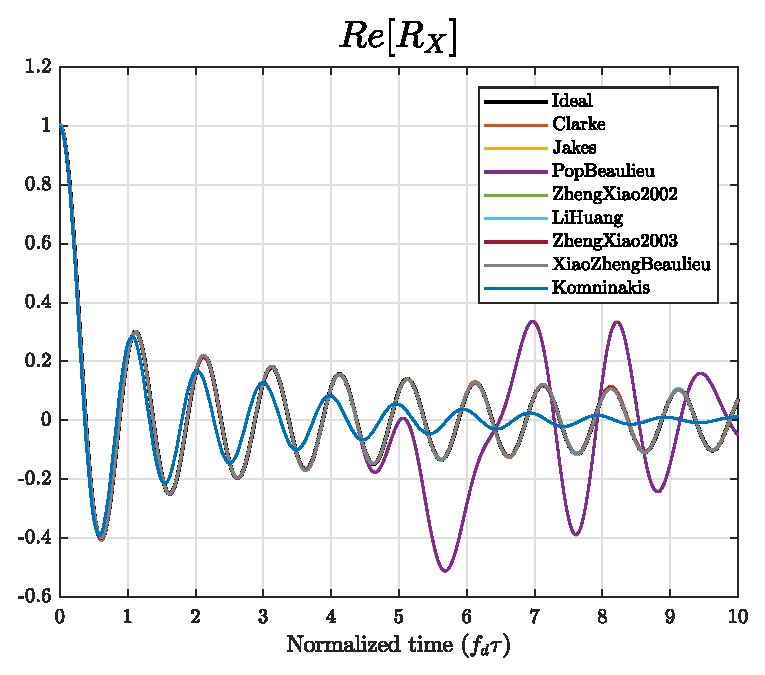
\includegraphics[width=\linewidth]{img/ReX.eps}
	\end{minipage}
	\hfill
	\begin{minipage}{.32\linewidth}
		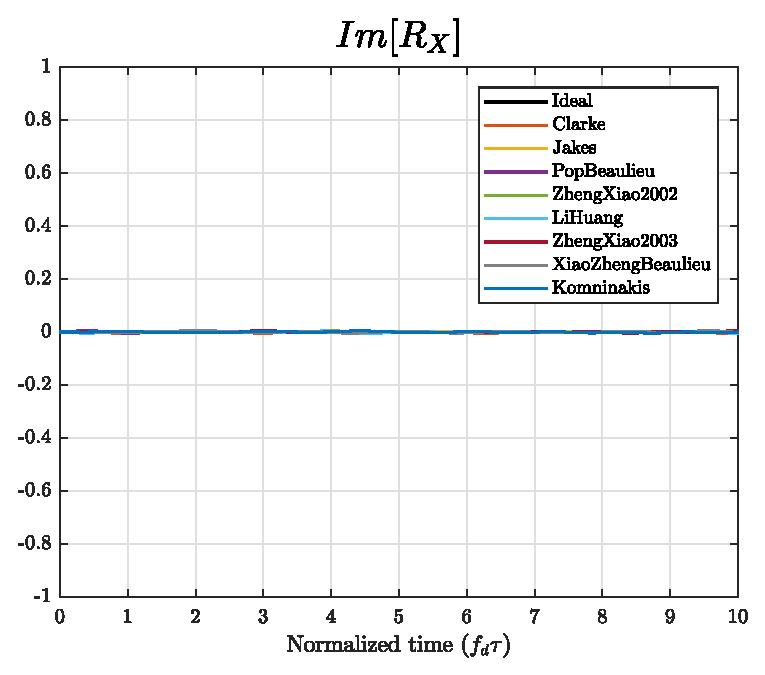
\includegraphics[width=\linewidth]{img/ImX.eps}
	\end{minipage}
	\hfill
	\begin{minipage}{.32\linewidth}
		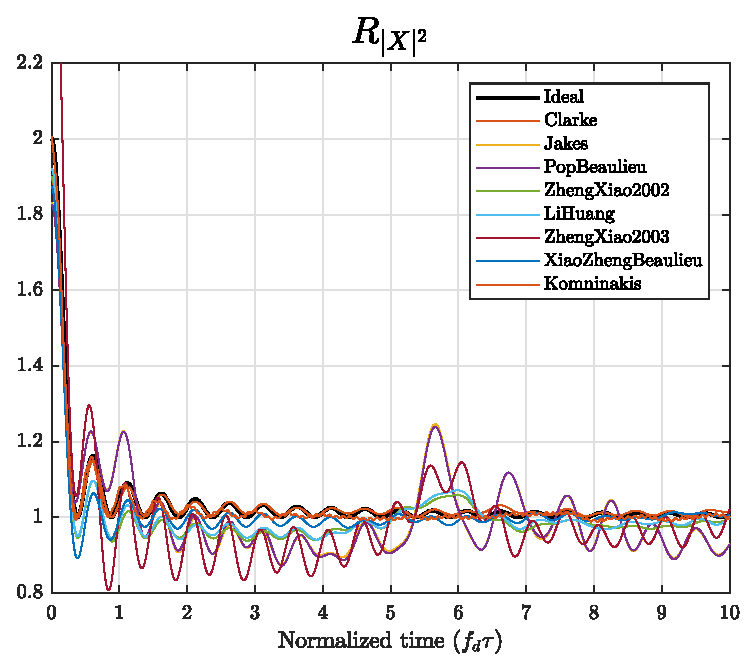
\includegraphics[width=\linewidth]{img/X2.eps}
	\end{minipage}
	\hfill
	
	\caption{Correlations of the channels}
	\label{fig:3xcorr}
\end{figure}

%%%%%%%%%%%%%%%%%%%%%%%%%%%%%%%%%%%%%%%%%%%%%%%%%%%%%%%%%%%%%%%%%%%%%%%%%%%%%%%%%%%%%%%%%%%%%%%
%%%%%%%%%%%% LCR/AFD
%%%%%%%%%%%%%%%%%%%%%%%%%%%%%%%%%%%%%%%%%%%%%%%%%%%%%%%%%%%%%%%%%%%%%%%%%%%%%%%%%%%%%%%%%%%%%%%
\begin{figure}
	\hfill
	\begin{minipage}{.45\linewidth}
		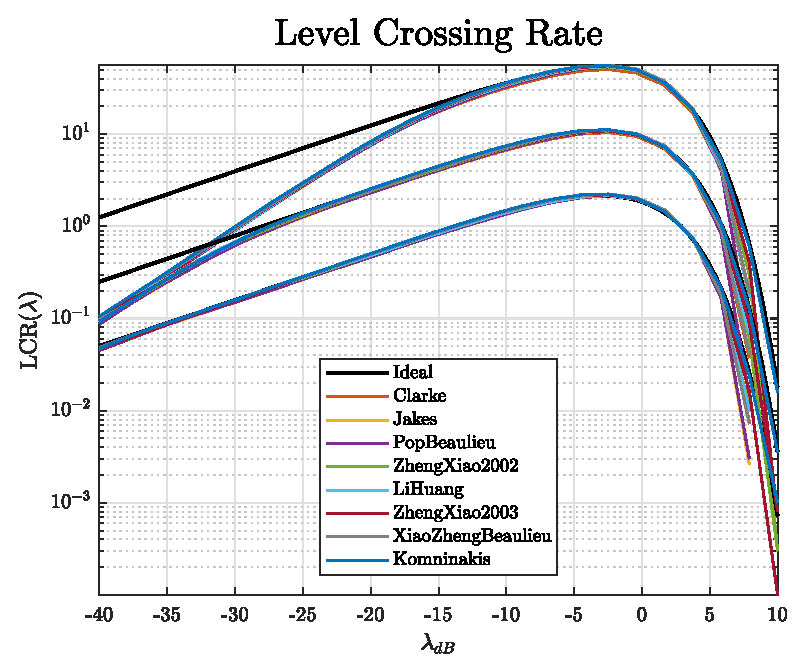
\includegraphics[width=\linewidth]{img/multiLCR.eps}
	\end{minipage}
	\hfill
	\begin{minipage}{.45\linewidth}
		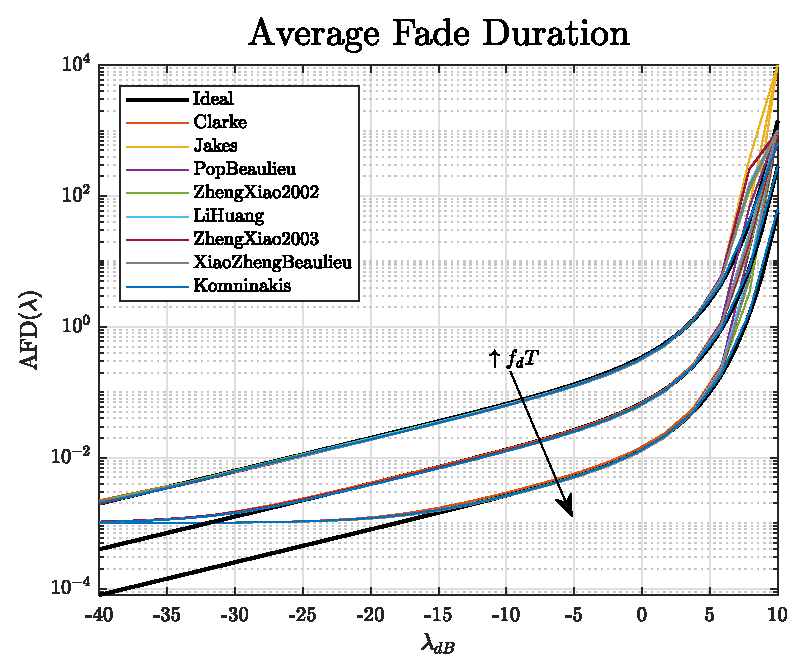
\includegraphics[width=\linewidth]{img/multiAFD.eps}
	\end{minipage}
	\hfill
	
	\caption{Plots for threshold-based statistics. Note that $\lambda_{dB} \triangleq 20\, \log_{10} \lambda$ since it's envelope related, not power related}
	\label{fig:LCR_AFD}
\end{figure}

%%%%%%%%%%%%%%%%%%%%%%%%%%%%%%%%%%%%%%%%%%%%%%%%%%%%%%%%%%%%%%%%%%%%%%%%%%%%%%%%%%%%%%%%%%%%%%%
%%%%%%%%%%%% Simulation Time
%%%%%%%%%%%%%%%%%%%%%%%%%%%%%%%%%%%%%%%%%%%%%%%%%%%%%%%%%%%%%%%%%%%%%%%%%%%%%%%%%%%%%%%%%%%%%%%
\begin{figure}
	\hfill
	\subfigure[Overall Simulation Time]{
		\includegraphics[width=.31\linewidth]{img/simTime.eps}
	}
	\hfill
	\subfigure[Kominakis Simulation Time]{
		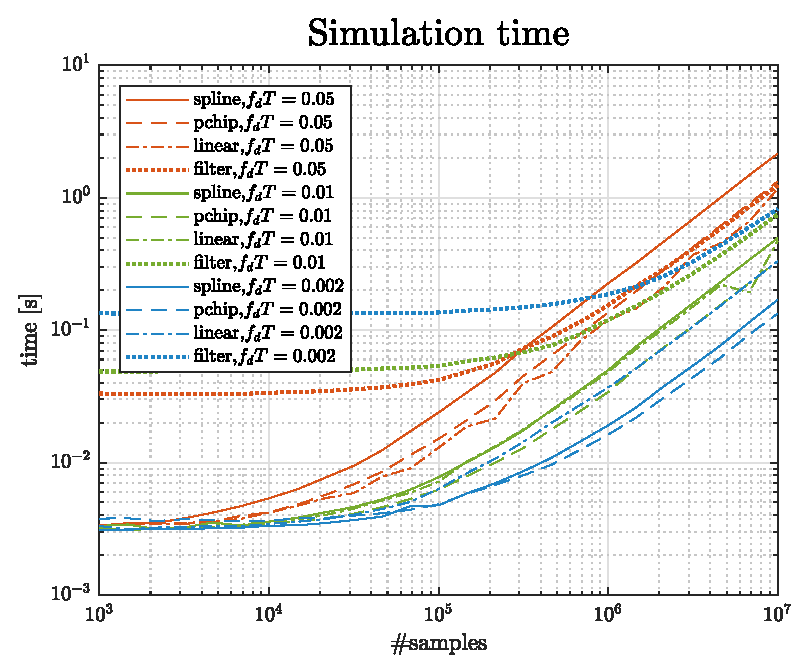
\includegraphics[width=.31\linewidth]{img/simTime_Komninakis.eps}
	}
	\hfill
	\subfigure[Simulation Time for different $N_{ch}$]{
		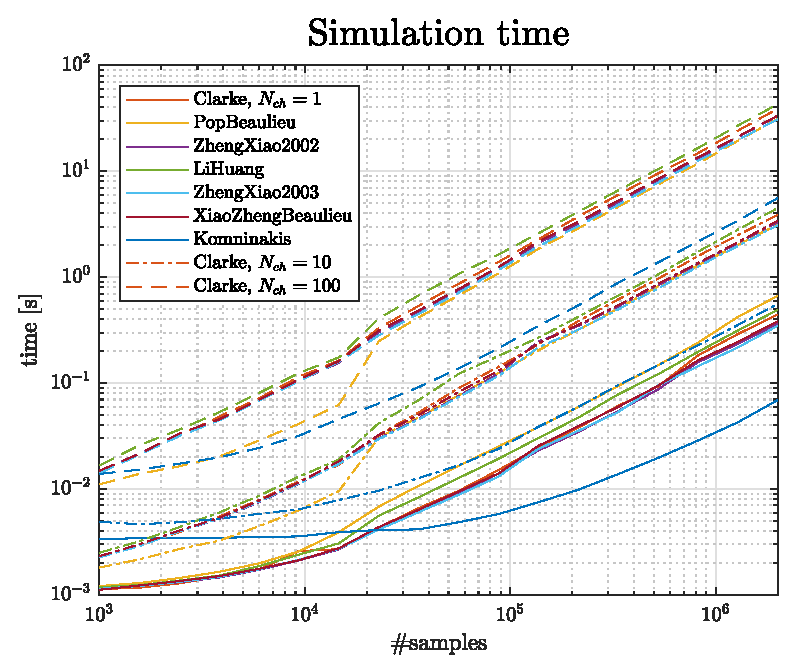
\includegraphics[width=.31\linewidth]{img/multiSimTime.eps}
	}
	\hfill
	
	\caption{Simulation time for current implementations}
	\label{fig:simTime}
\end{figure}
\section{Conclusions} % max 1/2 page
% Obj. 1: Summariza what you did in the project
% Obj. 2: Lessons learned
\label{sec:conclusions}




\nocite{*}
\printbibliography

\end{document}
